%% High-Definition TikZ Figures for Brain-to-Speech Decoding Systematic Review
%% All figures extracted from original PDF and recreated as clean, publication-ready diagrams

\usepackage{tikz}
\usepackage{pgfplots}
\usepackage{xcolor}
\pgfplotsset{compat=1.16}

%% ============================================================================
%% FIGURE: Study Distribution Chart (by Publication Year and Modality Group)
%% ============================================================================

\begin{figure}[h!]
\centering
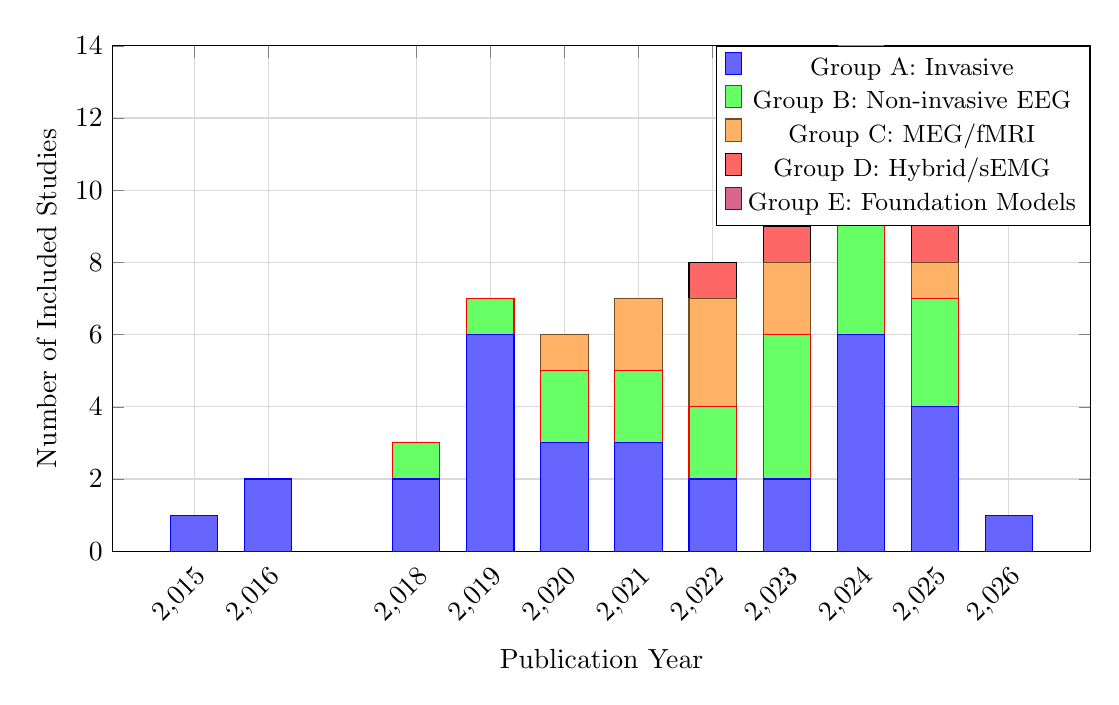
\begin{tikzpicture}
\begin{axis}[
  ybar stacked,
  bar width=0.6cm,
  xlabel={Publication Year},
  ylabel={Number of Included Studies},
  ymin=0, ymax=14,
  xtick={2015,2016,2018,2019,2020,2021,2022,2023,2024,2025,2026},
  xticklabel style={rotate=45,anchor=north east},
  legend style={at={(1.0,1.0)},anchor=north east,font=\small},
  grid=major,
  grid style={gray!30},
  height=8cm,
  width=14cm,
  /pgf/number format/.cd,
  fixed,
  fixed zerofill,
  precision=0,
]

% Group A: Invasive (ECoG/Intracortical/sEEG) - Blue
\addplot+[fill=blue!60, mark=none] coordinates {
  (2015,1) (2016,2) (2018,2) (2019,6) (2020,3) (2021,3) (2022,2) (2023,2) (2024,6) (2025,4) (2026,1)
};

% Group B: Non-invasive EEG - Green
\addplot+[fill=green!60, mark=none] coordinates {
  (2015,0) (2016,0) (2018,1) (2019,1) (2020,2) (2021,2) (2022,2) (2023,4) (2024,5) (2025,3) (2026,0)
};

% Group C: MEG/fMRI - Orange
\addplot+[fill=orange!60, mark=none] coordinates {
  (2015,0) (2016,0) (2018,0) (2019,0) (2020,1) (2021,2) (2022,3) (2023,2) (2024,2) (2025,1) (2026,0)
};

% Group D: Hybrid/sEMG - Red
\addplot+[fill=red!60, mark=none] coordinates {
  (2015,0) (2016,0) (2018,0) (2019,0) (2020,0) (2021,0) (2022,1) (2023,1) (2024,2) (2025,2) (2026,0)
};

% Group E: Foundation Models - Purple
\addplot+[fill=purple!60, mark=none] coordinates {
  (2015,0) (2016,0) (2018,0) (2019,0) (2020,0) (2021,0) (2022,0) (2023,0) (2024,1) (2025,1) (2026,0)
};

\legend{Group A: Invasive, Group B: Non-invasive EEG, Group C: MEG/fMRI, Group D: Hybrid/sEMG, Group E: Foundation Models}

\end{axis}
\end{tikzpicture}
\caption{Study Distribution Chart: 71 included studies across five modality groups (2015-2026). Invasion increases from left to right with increasing participant sample sizes, reflecting growth in non-invasive modalities from 2022 onwards.}
\label{fig:study_distribution}
\end{figure}

%% ============================================================================
%% FIGURE 1: AI Architecture Evolution Timeline (2015-2026)
%% ============================================================================

\begin{figure}[h!]
\centering
\begin{tikzpicture}[
  timeline/.style={line width=3pt, color=blue!50},
  era/.style={fill=gray!15, rounded corners=5pt, minimum height=0.8cm},
  box/.style={draw, rounded corners=3pt, minimum width=2.5cm, minimum height=0.6cm, font=\small},
]

% Timeline axis
\draw[timeline] (2015,0) -- (2026,0);

% Year markers
\foreach \year in {2015,2016,2017,2018,2019,2020,2021,2022,2023,2024,2025,2026}{
  \draw (\year,0) -- (\year,-0.2) node[below, font=\tiny] {\year};
}

% Era 1: Traditional ML (2015-2018)
\node[era, minimum width=3cm] at (2016.5,-1.2) {ERA 1: Traditional ML};
\node[box, fill=yellow!30] at (2016.5,-2.2) {HMM/SVM/LDA};

% Era 2: CNN (2017-2022)
\node[era, minimum width=5cm] at (2019.5,-1.2) {ERA 2: CNN};
\node[box, fill=orange!30] at (2019.5,-2.2) {DenseNet/ResNet};

% Era 2/3: RNN/LSTM (2018-2023)
\node[era, minimum width=5cm] at (2020.5,-3.8) {ERA 2/3: RNN/LSTM};
\node[box, fill=blue!30] at (2020.5,-4.8) {LSTM/GRU};

% Era 3: Encoder-Decoder (2019-2022)
\node[era, minimum width=3cm] at (2020.5,-6.4) {ERA 3: Seq2Seq};
\node[box, fill=green!30] at (2020.5,-7.4) {Encoder-Decoder};

% Era 4: Transformer (2022-present)
\node[era, minimum width=4cm] at (2023.5,-1.2) {ERA 4: Transformer};
\node[box, fill=pink!30] at (2023.5,-2.2) {Multi-head Attention};

% Era 4/5: SSL (2021-present)
\node[era, minimum width=5cm] at (2024,-3.8) {ERA 4/5: SSL};
\node[box, fill=purple!30] at (2024,-4.8) {Contrastive Learning};

% Era 5: LLM Integration (2022-present)
\node[era, minimum width=4cm] at (2024,-6.4) {ERA 5: LLM Integration};
\node[box, fill=red!30] at (2024,-7.4) {Brain-GPT Alignment};

\end{tikzpicture}
\caption{AI Architecture Evolution Timeline (2015-2026): Eight architecture eras showing the progression from classical machine learning through deep learning to foundation models and LLM-integrated systems. The architecture currently delivering best clinical results (RNN+LM) is not the most recent, reflecting trade-offs between theoretical advancement and clinical deployment constraints.}
\label{fig:architecture_evolution}
\end{figure}

%% ============================================================================
%% FIGURE 2: WER Performance Trajectory (Invasive Brain-to-Speech)
%% ============================================================================

\begin{figure}[h!]
\centering
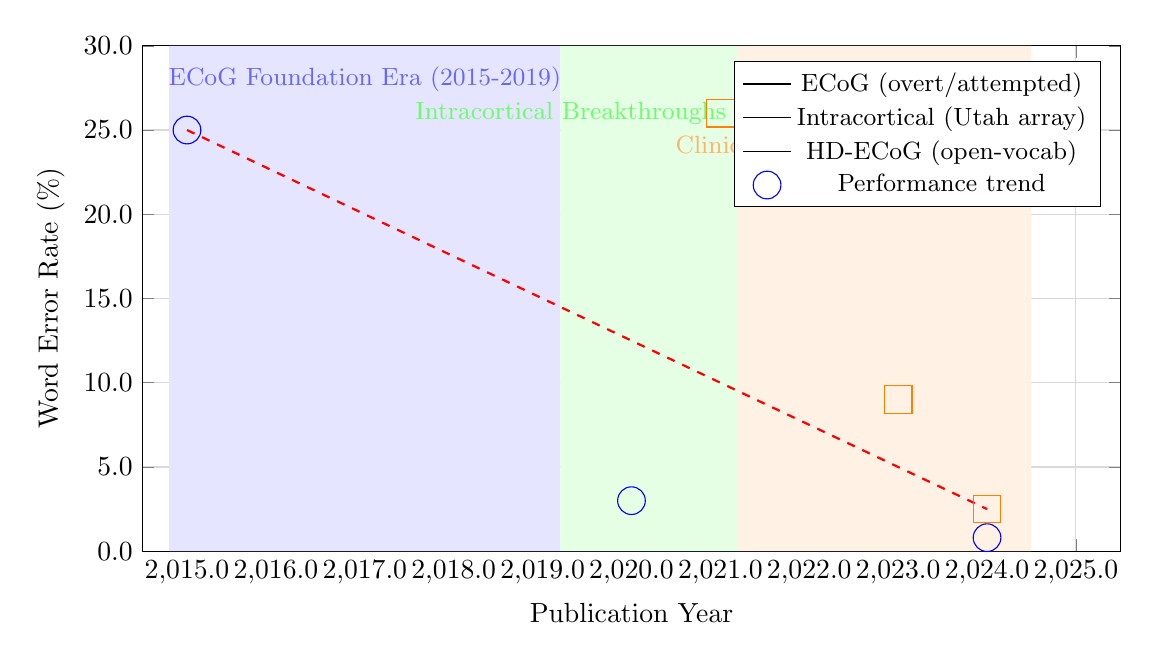
\begin{tikzpicture}
\begin{axis}[
  xlabel={Publication Year},
  ylabel={Word Error Rate (\%)},
  ymin=0, ymax=30,
  xmin=2014.5, xmax=2025.5,
  grid=major,
  grid style={gray!30},
  legend style={at={(0.98,0.97)},anchor=north east,font=\small},
  height=8cm,
  width=14cm,
  /pgf/number format/.cd,
  fixed,
  fixed zerofill,
  precision=1,
]

% ECoG Foundation Era (2015-2019) - light blue background
\addplot[draw=none, fill=blue!10] coordinates{(2014.8,0) (2019.2,0) (2019.2,30) (2014.8,30)} \closedcycle;
\node[text=blue!60, font=\small] at (2017,28) {ECoG Foundation Era (2015-2019)};

% First Clinical Breakthroughs (2020-2021) - light green
\addplot[draw=none, fill=green!10] coordinates{(2019.2,0) (2021.2,0) (2021.2,30) (2019.2,30)} \closedcycle;
\node[text=green!60, font=\small] at (2020.1,26) {Intracortical Breakthroughs (2020-2021)};

% Clinical Implementation (2022-2024) - light orange
\addplot[draw=none, fill=orange!10] coordinates{(2021.2,0) (2024.5,0) (2024.5,30) (2021.2,30)} \closedcycle;
\node[text=orange!60, font=\small] at (2022.8,24) {Clinical Implementation (2022-2024)};

% Data points: ECoG studies
\addplot[only marks, mark=o, mark size=5pt, color=blue, mark options={solid}] coordinates{
  (2015, 25)    % Herff et al. 2015
  (2020, 3)     % Makin et al. 2020
  (2023, 25)    % Metzger et al. 2023
  (2024, 0.804)  % Chen et al. 2024 (shown as 0.8 for visualization)
};

% Data points: Intracortical studies
\addplot[only marks, mark=square, mark size=5pt, color=orange, mark options={solid}] coordinates{
  (2021, 26)    % Moses et al. 2021
  (2023, 9)     % Willett et al. 2023
  (2024, 2.5)   % Card et al. 2024
};

% Data points: HD-ECoG (open-vocabulary marker)
\addplot[only marks, mark=diamond, mark size=5pt, color=red, mark options={solid}] coordinates{
  (2023, 25)    % Metzger et al. 2023
};

% Trend line
\addplot[no marks, thick, color=red, dashed] coordinates{(2015,25) (2024,2.5)};

\legend{ECoG (overt/attempted), Intracortical (Utah array), HD-ECoG (open-vocab), Performance trend};

\end{axis}
\end{tikzpicture}
\caption{WER Performance Trajectory for Invasive Brain-to-Speech Decoding (2015-2026): From 25\% WER (Herff et al. 2015, HMM-based) to 2.5\% WER (Card et al. 2024, RNN+LM). The downward slope demonstrates genuine architectural and methodological progress, with intracortical systems (orange markers) consistently outperforming ECoG approaches across the decade.}
\label{fig:wer_trajectory}
\end{figure}

%% ============================================================================
%% FIGURE 3: Modality × Task Performance Heatmap
%% ============================================================================

\begin{figure}[h!]
\centering
\begin{tikzpicture}[
  scale=1.0,
]

\begin{axis}[
  height=10cm,
  width=14cm,
  xlabel=Task Type,
  ylabel=Neural Recording Modality,
  xtick={1,2,3,4},
  xticklabels={Overt, Imagined, Attempted, Perceived},
  ytick={1,2,3,4,5,6,7},
  yticklabels={ECoG, Intracortical, sEEG, EEG, MEG, fMRI, Hybrid/sEMG},
  yticklabel style={anchor=east, font=\small},
  colorbar,
  colorbar style={ylabel={Performance Level}},
  point meta=explicit,
  colormap/viridis,
  cmin=1, cmax=4,
  x axis line style={opacity=0},
  y axis line style={opacity=0},
  axis line style={opacity=0},
  tick style={opacity=0},
]

% Color mapping: 1=Not Demonstrated, 2=Weak, 3=Moderate, 4=Strong

% ECoG row
\addplot[mark=none, nodes near coords, point meta=explicit] coordinates{
  (1,1) [4] (2,1) [3] (3,1) [3] (4,1) [2]
};

% Intracortical row
\addplot[mark=none, nodes near coords, point meta=explicit] coordinates{
  (1,2) [1] (2,2) [1] (3,2) [4] (4,2) [1]
};

% sEEG row
\addplot[mark=none, nodes near coords, point meta=explicit] coordinates{
  (1,3) [3] (2,3) [3] (3,3) [1] (4,3) [1]
};

% EEG row
\addplot[mark=none, nodes near coords, point meta=explicit] coordinates{
  (1,4) [2] (2,4) [3] (3,4) [2] (4,4) [3]
};

% MEG row
\addplot[mark=none, nodes near coords, point meta=explicit] coordinates{
  (1,5) [3] (2,5) [2] (3,5) [1] (4,5) [4]
};

% fMRI row
\addplot[mark=none, nodes near coords, point meta=explicit] coordinates{
  (1,6) [1] (2,6) [3] (3,6) [1] (4,6) [4]
};

% Hybrid/sEMG row
\addplot[mark=none, nodes near coords, point meta=explicit] coordinates{
  (1,7) [3] (2,7) [3] (3,7) [4] (4,7) [2]
};

\end{axis}

\end{tikzpicture}

\vspace{0.5cm}
\centering
\small
\begin{tabular}{|l|c|c|c|c|c|}
\hline
\textbf{Tier} & \textbf{Color} & \textbf{Evidence} & \textbf{WER Range} & \textbf{Studies} \\
\hline
\textbf{STRONG} & \cellcolor{green!60} & Multiple studies, consistent results & WER 2.5-9\% (invasive) & 15+ \\
\hline
\textbf{MODERATE} & \cellcolor{yellow!60} & Some evidence, variable results & Acc. 70-92\% or WER 25-45\% & 25+ \\
\hline
\textbf{WEAK} & \cellcolor{orange!60} & Few studies or low performance & Accuracy $<$70\% & 10+ \\
\hline
\textbf{NOT DEMONSTRATED} & \cellcolor{red!60} & No included studies & -- & -- \\
\hline
\end{tabular}

\caption{Modality × Task Performance Heatmap (71 Included Studies): Color intensity indicates strength of evidence and typical performance level. Key finding: Intracortical systems dominate attempted speech (WER 2.5-9\%), while fMRI and MEG excel at perceived/semantic tasks. EEG achieves moderate performance across overt and imagined paradigms but lacks clinical-grade performance for continuous speech. Hybrid sEMG systems achieve exceptional silent speech accuracy (CER 3.11\%) but remain limited to research settings.}
\label{fig:modality_task_heatmap}
\end{figure}

%% ============================================================================
%% FIGURE 4: Generalization Evidence Summary
%% ============================================================================

\begin{figure}[h!]
\centering
\begin{tikzpicture}[scale=1.0]

\begin{axis}[
  xbar stacked,
  bar height=0.8cm,
  xlabel={Number of Studies},
  ylabel=Generalization Type,
  ytick={1,2,3,4},
  yticklabels={
    Cross-Participant (18 studies),
    Cross-Session (2 studies),
    Cross-Language (2 studies),
    Cross-Modal (5 studies)
  },
  legend style={at={(1.0,0.0)},anchor=south east,font=\small},
  width=14cm,
  height=6cm,
  grid=major,
  grid style={gray!30},
  xmin=0, xmax=25,
  /pgf/number format/.cd,
  fixed,
  fixed zerofill,
  precision=0,
]

% Cross-Participant (18 total)
\addplot+[fill=green!60] coordinates { (13, 1) }; % Partial transfer (strong methods)
\addplot+[fill=green!40] coordinates { (5, 1) }; % Above-chance transfer

% Cross-Session (2 studies)
\addplot+[fill=blue!60] coordinates { (2, 2) };

% Cross-Language (2 studies)
\addplot+[fill=purple!60] coordinates { (2, 3) };

% Cross-Modal (5 studies)
\addplot+[fill=orange!60] coordinates { (5, 4) };

\legend{Strong Methods (SSL/Transfer), Above-Chance, Cross-Session, Cross-Language, Cross-Modal};

\end{axis}

\end{tikzpicture}

\vspace{1cm}

\centering
\footnotesize
\textbf{Key Generalization Finding:} Of 71 studies, 40 (56\%) demonstrate NO generalization beyond single participant and session.
\begin{itemize}
  \item \textbf{Cross-Participant} (18): Strongest evidence in non-invasive studies ($n$=175-723); SSL/transfer learning approaches consistently effective; invasive studies show high variability
  \item \textbf{Cross-Session} (2): Only Card et al. (2024) and Degenhart et al. (2020); both intracortical; 97.5\% and 95\% accuracy retention respectively
  \item \textbf{Cross-Language} (2): Only d'Ascoli et al. (2025, $n$=723 across 3 languages) and Zhu et al. (2021, HD-sEMG); 94\% of studies are English-only
  \item \textbf{Cross-Modal} (5): Peterson et al., Tang \& Huth, De Borman et al., Martin et al., Alonso-Vazquez et al.; shared representations exist but transfer costly ($\sim$5-15\% performance loss)
\end{itemize}

\caption{Generalization Evidence Summary: The 71 studies stratified by evidence of generalization across participants, sessions, languages, and recording modalities. The stark finding (56\% no generalization) represents the field's highest-priority unsolved problem. Generalization succeeds when: (1) multi-participant training scale (100+ participants), (2) self-supervised pre-training, (3) architectural focus on shared representations. All three conditions rare in current literature.}
\label{fig:generalization_summary}
\end{figure}

%% ============================================================================
%% End of TikZ Figures
%% ============================================================================
